\chapter{M-files Used in This Research}\appcaption{Appendix A}

\section{M-files for System Identification and Control Design}

\tab The empirical model building and controller design were done using Matlab. During this
research, three Matlab m-files were used to automate the system identification and control
design procedures. These m-file were

\begin{description}
	\item[id\_arm ax.m] - Identifies various order ARMAX model based on input-output data.
	\item[ctrldsgn .m] - Designs controllers based upon the LQG/LTR technique and performs model reduction.
	\item[ctrlsat.m] - Adds anti-windup logic to a controller designed with ctrldsgn.
\end{description}

\newpage

\subsection{id\_armax.m}

\begin{lstlisting}[gobble=4]
	function [th,simout]=id_armax(z,dt,order,delay,filename,plots,pauses);
	%%%%%%%%%%%%%%%%%%%%%%%%%%%%%%%%%%%%%%%%%%%%%%%%%%%%%%%%%%%%%%%%%%
	%
	%Descritpion: id_armax takes input-output data and identifies various order armax models and writes the results to filename.diary
	%
	%Parameter List:
	%
	%	Inputs:
	%			z:		the input/output data to be used for identification in the form: z = [output, input]
	%			dt:		the sampling period for the data
	%			order:	vector containing the order models to be identified
	%			delay:	pure time delay, in samples, present in data
	%			filename: file name for diary and plots (id_armax will
	%					automatically add extension)
	%			plots: 
	%					0 - don't save plots to files
	%					1 - save plots to files
	%			pauses:
	%					0 - no pause in program
	%					1 - pauses after each plot
	%
	%	Outputs:
	%			th:		th-format model for last identified order
	%			simpout:	matrix containing simulated output for each order
	%
	%%%%%%%%%%%%%%%%%%%%%%%%%%%%%%%%%%%%%%%%%%%%%%%%%%%%%%%%%%%%%%%%%%
	
	%
	% set default arguments
	%
	if nargin < 7, pauses = 0; end;
	if nargin < 6, plots = 0; end;
	if nargin < 5, filename = 'junk'; end;
	if nargin < 4, delay = 1; end;
	
	%
	% Plot Neasured Response
	%
	y = z(:,1);
	[xs,ys] = size(z);
	t = dt*[0:xs-1]';
	plot(t,z(:,1)),grid;
	title(['Measured Response of System'])
	xlabel('Time (seconds)')
	ylabel('Output')
	
	if plots == 1,
	plotfile = [filename,'.actual.ps'];
	diary on
	disp(['Printing Plot of Measured Response in file ', plotfile])
	diary off
	eval(['print ', plotfile]);
	end % End If - Print Plot
	
	if pauses == 1, disp('Hit Any Key to Continue'),pause, end
	
	%
	% Start Identification
	%
	
	for j = 1:max(size(order)), % Loop through for each element in order
		
		i = order(j);
		th = armax(z,[i i i delay],50,-1,-1,-1,dt);
		
		eval(['diary ', filename,'.diary']);
		disp(['Theta - Armax Model -  Order ',int2str(i)])
		disp(['--------------------------------'])
		disp([' '])
		present(th)
		diary off
		
	% Evaluate System
		
		na = [1:i];
		nb = [i+1:2*i];
		a  = [1 th(3,na)];
		b  = [th(3,nb)];
		[bc,fc] = contin(tj,1,1);
		
		diary on
		disp(' ')
		disp('Discrete G(z)')
		disp('Numerator')
		disp(b)
		disp('Denominator')
		disp(a)
		disp('Zeros')
		disp(roots(b))
		disp('Poles')
		disp(roots(a))
		disp(' ')
		disp('Continuous G(s)')
		disp('Numerator')
		disp(bc)
		disp('Denominator')
		disp(fc)
		disp('DC gain')
		disp(polyval(bc,0)/polyval(fc,0))
		disp('Zeros')
		disp(roots(bc))
		disp('Poles')
		disp(roots(fc))
		disp(['delay = ' int2str(delay)])
		disp(' ')
		disp(' ')
		diary off
		
		[mag(:i) phase(:,i)] = bode(bc,fc,logspace(-3,3,200));
		loss(j) = th(1,1);
	
	%
	% Simulate System with Identified Theta
	%
		[ysim] = idsim(z(:2),th);
		
		plot(t,ysim,t,z(:,1),'y
		:');
		grid;
		title(['Measured and Simulated Response of Order ',int2str(i), ...
			' ARMAX Model'])
		xlabel('Time (seconds)')
		ylabel('Simulated Output')
		legend('Simulated Response','Actual Response')
		simout(:,j) = ysim;
		
		if plots == 1,
			plotfile = [filename,'.sim',int2str(i),'.ps'];
			diary on
			disp(['Printing Simulated response of Order ',int2str(i), ...
				' in file ', plotfile])
			diary off
			eval(['print ', plotfile]);
		end % End If - Print Plot
		
		
		if pauses == 1, disp('Hit Any Key to Continue'),pause, end
	
	%
	% Find Resuduals
	%
		titl = ['Correlation of Residuals for Order ',int2str(i),' ARMAX Model'];
		[e,r] = resid2(z,th,titl);
		
		
		if plots == 1,
			plotfile = [filename,'.resid',int2str(i),'.ps'];
			diary on
			disp(['Printing resid for Order ',int2str(i),' in file ', plotfile])
			disp(' ')
			diary off
			eval(['print ', plotfile]);
		end % End If - Print Plots
	end % End For Loop
	
	if pauses == 1, disp('Hit Any Key to Continue'),pause, end
	
	%
	% bode
	%
	
	subplot([211])
	loglog(logspace(-3,3,200),mag)
	title(['Bode pplots of orders [' int2str(order) ']'])
	ylavel('mag'), xlabel('rad/sec'), grid
	subplot([212])
	semilogx(logspace(-3,3,200),phase)
	ylabel('phase'), xlabel('rad/sec'), grid
	
	if plots == 1,
	plotfile = [filename,'.bode.ps'];
	diary on
	disp(['Printing bode for orders[',int2str(order), ...
				'] infile ', plotfile])
	disp(' ')
	diary off
	eval(['print ', plotfile]);
	end % End if - Print Plots
	
	%
	% Log Loss Functions
	%
	format short e
	diary on
	disp(['		Order 		Loss Function'])
	disp([order',loss']);
	diary off
	format short
	
	end;

\end{lstlisting}

\newpage

\subsection{ctrldsgn.m}

\begin{lstlisting}[gobble=4]
	function [Acr,Bcr,Ccr,Dcr] = ctrldsgn(Ap,Bp,Cp,Dp,alpha,Qq,Rr,rho)
	%%%%%%%%%%%%%%%%%%%%%%%%%%%%%%%%%%%%%%%%%%%%%%%%%%%%%%%%%%%%%%%%%%
	%
	% Description: LQG/LTR controller design with model reduction
	%
	% Parameter List:
	%
	%		Inputs:
	%					[Ap,Bp,Cp,Dp] - state space representation of the plant
	%			
	%				LQR Design
	%					State weights Q = [alpha*Cp'*Cp,zeros(ns,no);zeros(no,ns),Qq];
	%					Input Weights R = Ru;
	%
	%				LQG/LTR Design
	%								W = Bp*Bp'
	%								V = rho*I
	%
	%		Outputs:
	%				[Acr,Bcr,Ccr,Dcr] - state space representation of the reduced order control
	%%%%%%%%%%%%%%%%%%%%%%%%%%%%%%%%%%%%%%%%%%%%%%%%%%%%%%%%%%%%%%%%%%
	
	w = logspace(-2,2);
	time = [0:1/20:40];
	
	%
	% Determine size of plant
	%
	
	[ns,ni] = size(Bp);
	[no,ns] = size(Cp);
	
	%
	% Augment thhe plant with integrators
	%
	%		\dot{x} = Ap x + Bp u
	%		\dot{q} = y - r
	%			y = Cp x
	%
	
	Am = [Ap, zeros(ns,no); Cp, zeros(no,no)];
	Bm = [Bp; zeros(no,no)];
	Cm = [Cp, zeros(no,no)];
	Dm = zeros(no,ni);
	
	%
	% LQR Design
	%
	
	Q = [alpha*Cp'*Cp, zeros(ns,no); zeros(no,ns), Qq];
	R = Rr;
	[K,S] = lqr(Am,Bm,Q,R);
	
	%
	% Analysis of LQR Design
	%
	%		Loop Gain of hte State Feedback Design
	%
	
	for i = 1:ni,
		str = ['Loop Gain: Input ',num2str(i)];
		[mag,ph] = mbode(Am,Bm,-K,Dm,i,i,w,str);
		disp('Hit Any Key To Continue');
		pause;
	end
	
	%
	%		Step Response for Closed Loop System
	%
	
	Asf = [Am-Bm*K];
	Bsf = [zeros(ns,ni); -eye(ni)];
	Csf = Cm;
	Dsf = Dm;
	
	for i=1:ni,
		y = step(Asf,Bsf,Csf,Dsf,i,time);
		titl = ['Response of outputs to a step in reference ',num2str(i)];
		for j = 1:no,
			subplot(no,1,j), plot(time,y(:,j)),grid
			if j == 1, title(titl), end
			xlabel('Time (seconds)');
			ylabel(['Output ',num2str(j)]);
		end
		keyboard
		
		u = step(Asf,Bsf,-K,Dsf,i,time);
		titl = ['Response of inputs to a step in reference ',num2str(i)];
		for j = 1:ni,
			subplot(ni,1,j), plot(time,u(:,j)),grid
			if j == 1, title(titl), end
			xlabel('Time (seconds)');
			ylabel(['Input ',num2str(j)]);
		end
		keyboard
	end
	
	%
	%	Loop Transfer Recovery
	%
	
	[L,Y] = lqr(Ap',Cp',Bp*Bp',rho*eye(no));
	
	nas = ns+no;
	
	K1 = K(:,1:ns);
	K2 = K(:,ns+1:nas);
	
	Ac = [Ap-Bp*K1-L'*Cp, -Bp*K2; zeros(no,nas)];
	Bc = [L', zeros(ns,no); eye(no), -eye(no)];
	Cc = -L;
	Dc = zeros(ni,2*no);
	
	
	%
	%	Loop Gain at Output
	%
	
	Ao = [Ac, zeros(nas,ns); Bp*Cc, Ap];
	Bo = [L'; eye(no);zeros(ns,no)];
	Co = [zeros(no,nas), Cp];
	Do = zeos(no,no);
	
	for i = 1:no,
		str = ['Loop Gain: Output ',num2str(i)];
		[mag,ph] = mbode(Ao,Bo,Co,Do,i,i,w,str);
		keyboard
	%	disp('Hit Any Key To Continue');
	%	pause;
	end
	
	%
	%	Closed Loop System
	%
	
	Acl = [Ac, [L';eye(no)]*Cp; Bp*Cc, Ap]l
	Bcl = [zeros(ns,np);-eye(no),zeros(ns,no)];
	Ccl = [zeros(no,nas), Vp];
	Dcl = zeros(no,no);
	
	for i=1:ni,
		y = step(Act,Bcl,Ccl,Dcl,i,time);
		titl = ['Response of outputs to a step in reference ',num2str(i)];
		for j = 1:no,
			subplot(no,1,j), plot(time,y(:j)),grid
			if j == 1, title(titl), end
			xlabel('Time (seconds)');
			ylabel(['Output',num2str(j)]);
		end
	  disp('Keyboard Cmds - type return to continue')
	  keyboard
	
		u = step(Acl,Bcla,[-K,zeros(ni,ns)],Dcl,i,time);
		titl = ['Response of inputs to a step in reference ',num2str(i)]l
		for j = 1:ni,
			subplot(ni,1,j), plot(time,u(:,j)),grid
			if j == 1, title(titl), end
			xlabel('Time (seconds)');
			ylabel(['Input ',num2str(j)]);
		end
	  disp('Keyboard Cmds - type return to contine')
	  keyboard
	
	end
	
	disp('Calculating BalReal');
	%
	%	Balanced Realization
	%
	
	Ae = Ap-Bp*K1-L'*Cp;
	Be = [Bp, L'];
	Ce = -K1;
	De = [eye(no), zeros(ni,no)];
	
	Ai = zeros(no,no);
	Bi = [eye(no), -eye(no)];
	Ci = [-K2; zeros(no,no)]l
	Di = [zeros(no,2*no); eye(no), zeros(no,no)];
	
	[Ab,Bb,Cb,G,T] = balreal(Ae,Be,Ce);
	disp('Singular Values of (Ab,Bb,Cb)');
	disp(G)
	nsk = input('Enter number of states to keep: ','s');
	nk = str2num(nsk);

	%
	%	Controller Model Reduction
	%
	
	elim = [nk+1:length(G)];
	[Ar,Br,Cr,Dr] = modred(Ab,Bb,Cb,De,elim);
	[nsr,ni] = size(Br);
	
	Acr = [Ar, Br*Ci; zeros(no,nsr), zeros(no,no)];
	Bcr = [Br*Di; eye(no), -eye(no)];
	Ccr = [Cr, Dr*Ci];
	Dcr = [Dr*Di];
	
	
	Aro = [Acr, zeros(nsr+no,ns); Bp*Ccr, Ap];
	Bro = [Bcr(:,[1,no]);zeros(ns,no)];
	Cro - [zeros(no,nsr+no), Cp];
	Dro = zeros(no,no);
	
	for i = 1:no,
		clg;
		[mag,ph] = bode(Ac,Bc,Cc,Dc,i,w);
		[magr,phr] = bode(Acr,Bcr,Ccr,Dcr,i,w);
		mag = 20*log10(mag);
		magr = 20*log10(magr);
		
		for j = 1:no,
			subplot(no,1,j),semilogx(w,mag(:,j),'-',w,magr(:j),'--'),grid
			if j==1,12=legend('Full order','Reduced Order'),end;
		end
	
	disp('Keyboard Cmds - type return to continue')
	keyboard
	
	end
	
\end{lstlisting}

\newpage

\subsection{ctrlsat.m}

\begin{lstlisting}[gobble=4]
	function [au,bu,cu,du,ku] = ctrlsat(ac,bc,cc,dc,Qu,ru)
	%%%%%%%%%%%%%%%%%%%%%%%%%%%%%%%%%%%%%%%%%%%%%%%%%%%%%%%%%%%%%%%%%%
	%
	%	Description: Add anti-windup logic to controller
	%
	%	Parameter List:
	%
	%		Inputs:	
	%				[ac,bc,cc,dc]		controller
	%				Qu					state weights
	%				Ru					command error weights
	%		Outputs:
	%				 [au,bu,cu,du]		anti-windup controller
	%				 ku					anti-windup gain
	%				
	%%%%%%%%%%%%%%%%%%%%%%%%%%%%%%%%%%%%%%%%%%%%%%%%%%%%%%%%%%%%%%%%%%
	
	ku = lqr(ac',cc',Qu,Ru);
	ku = ku';
	
	[ci,cj] = size(cc);
	
	au = ac-ku*cc;
	bu = [bc-ku*dc ku];
	cu = cc;
	du = [dc 0*eye(ci)];
	
	disp(ku)
	
	end
	
\end{lstlisting}

\begin{figure}[H]
	\centering
	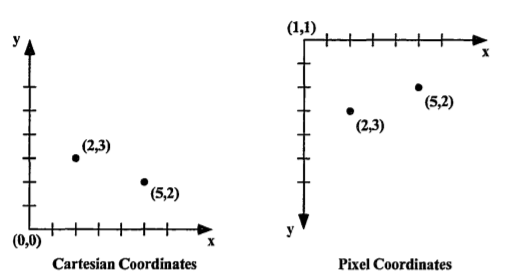
\includegraphics[scale = .8]{Figure A.1}
	\bf\caption{ Cartesian and pixel coordinate systems.}
	\label{fig:A.1}
\end{figure}

\section{M-files for Extraction of Sidewall Profile}

\tab The Matlab Image Processing Toolbox was used to analyze the SEM images. The first
step was to extract the areas of greatest intensity gradient using the edge command. This
command produces an binary image matrix (with element of either 0 or 1) with the edge
denoted with I ’s. This matrix used the pixel coordinate system shown in Figure A.l. A
plot of the image m atrix for the edge of the SEM image in Figure 5.22 is shown in Figure
A.2. A series of custom m-files were used to extract the etch profile from the image matrix. 

These m-files were

\begin{description}
	\item[clpt.m] - Returns the Cartesian coordinates of a point selected with the mouse,
	\item[edfill.m] - Fills in gaps in the edge profile.
	
	\begin{figure}[H]
		\centering
		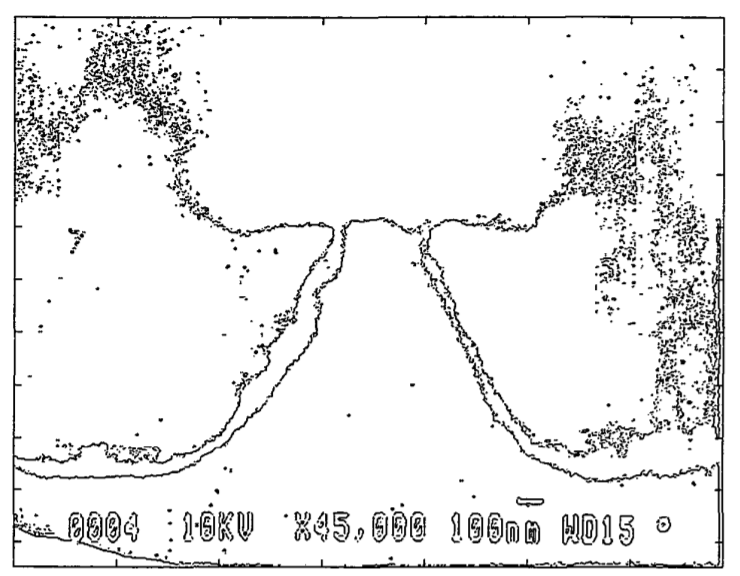
\includegraphics[scale = 0.5]{Figure A.2}
		\bf\caption{Edge Profile}
		\label{fig:A.2}
	\end{figure}
	
	\item[edscale.m] - Scales the image matrix from pixels to microns.
	\item[edshow.m] - Returns Cartesian coordinates of edges from image matrix.
	\item[mat2pic.m] - Converts from Cartesian coordinates to pixel coordinates.
	\item[pic2mat.m] - Converts from pixel coordinates to Cartesian coordinates,
	\item[snake.m] - Extracts specific edge profile from the image matrix.
\end{description}

\subsection{clpt.m}

\begin{lstlisting}
	function [i,j] = clpt(BW);
	%%%%%%%%%%%%%%%%%%%%%%%%%%%%%%%%%%%%%%%%%%%%%%%%%%%%%%%%%
	%
	%	Description: Return cartesian coordinates of points selected with mouse
	%
	%	Parameter List:
	%
	%		Inputs:
	%				BW = matrix containing edge image
	%
	%		Outputs:
	%				[i,j] = selected points in cartesian coordinates
	%
	%	Subfunctions:
	%			pic2mat.m
	%			mat2pic.m
	%
	%%%%%%%%%%%%%%%%%%%%%%%%%%%%%%%%%%%%%%%%%%%%%%%%%%%%%%%%%
	
	[si,sj] = size(BW);
	[gx,gy] = ginput(1);
	
	gx = floor(gx);
	gy = floor(gy);
	
	[gi,gj] = pic2mat(gx,gy,si,sj);
	
	found = 0;
	
	if BW(gi,gj) == 1,
	i = gi;
	j = gj;
		else
	R = 1;
	while found == 0
	theta = 0;
				while (theta < 2*pi) & (found == 0),
	i = round(gi + R*cos(theta));
					j = round(gj - R*sin(theta));
	[xtest,ytest] = mat2pic(i,j,si,sj);
	if BW(i,j) == 1,
	found = 1;
		else
	Theta = theta+(pi/20);
	end
	end
	R = R+1;
	end
	end
	
	end
	
\end{lstlisting}

\newpage 

\subsection{edfill.m}

\begin{lstlisting}
	function [BW2] = edfill(BW);
	%%%%%%%%%%%%%%%%%%%%%%%%%%%%%%%%%%%%%%%%%%%%%%%%%%%%%%%%%
	%
	%	Descritption: Fill in gaps in the edge profile image
	%
	%	Parameter List:
	%
	%		Inputs:
	%				BW = matrix containg edge image
	%		Outputs:
	%				BW2 = new image matrix
	%
	%	Subfunction:
	%		clpt.m
	%		edshow.m
	%%%%%%%%%%%%%%%%%%%%%%%%%%%%%%%%%%%%%%%%%%%%%%%%%%%%%%%%%
	
	edshow(BW);
	
	BW2 = BW;
	
	disp('Select First Point')
	
	[i1,j1] = clpt(BW);
	
	disp('Select Second Point')
	
	[i2,j2] = clpt(BW);
	
	i2-i1
	j2-j1
	
	if abs(i2-i1) > abs(j2-j1),
	
		v = polyfit([i1,i2],[j1,j2],1);
		
		imin = min(i1,i2);
		imax = max(i1,i2);
		
		x = [imin:imax]';
		
		y = round(polyval(v,x));
		
		for k = 1:length(x);
			BW2(x(k),y(k))=1;
		end
		
	else
	
		v = polyfit([j1,j2],[i1,i2],1);
		
		jmin = min(j1,j2);
		jmax = max(j1,j2);
		
		y = [jmin:jmax]';
		
		x = round(polyval(v,y));
		
		for k = 1:length(x);
			BW2(x(k),y(k))=1;
		end
		
	end
	
	edshow(BW2);
	
	end
	
\end{lstlisting}

\newpage

\subsection{edscale.m}

\begin{lstlisting}
	function [cent,scale] = edscale(BW);
	%%%%%%%%%%%%%%%%%%%%%%%%%%%%%%%%%%%%%%%%%%%%%%%%%%%%%%%%%
	%
	%	Description: Find scale factors from pixels to microns
	%
	%	Parameter List:
	%
	%		Inputs:
	%			BW = matrix containing edge image
	%
	%		Outputs:
	%			cent = origin for scaled image
	%			scale = scale factor from pixels to microns
	%
	%	Subfunctions:
	%		edshow.m
	%		clpt.m
	%
	%%%%%%%%%%%%%%%%%%%%%%%%%%%%%%%%%%%%%%%%%%%%%%%%%%%%%%%%%
	
	function [cent,scale] = edscale(BW);
	
	edshow(BW);
	
	disp('Select Center Point')
	[ic,jc] = ginput(1);
	cent = [ic,jc];
	
	disp('Select First Point')
	[i1,j1] = clpt(BW);
	
	disp('Select Second Point')
	[i2,j2] = clpt(BW);
	
	sc = input('Enter distance between pts. 1 and 2: ','s');
	
	dist = sqrt((i2-i1)^2 + (j2-j1)^2);
	scale = str2num(sc)/dist;
	
	end
	
\end{lstlisting}

\newpage

\subsection{edshow.m}

\begin{lstlisting}
	function [x,y]=edshow(BW);
	%%%%%%%%%%%%%%%%%%%%%%%%%%%%%%%%%%%%%%%%%%%%%%%%%%%%%%%%%
	%
	%	Description: Plot a edge detection image in cartesian (pic) coordinates
	%
	%	Parameter List:
	%
	%		Inputs:
	%			BW = matrix containing edge image
	%
	%		Outputs:
	%			[x,y] = coordinates (pic) of each pixel = 1 in matrix
	%
	%	Subfunctions: mat2pic.m
	%
	%%%%%%%%%%%%%%%%%%%%%%%%%%%%%%%%%%%%%%%%%%%%%%%%%%%%%%%%%
	
	[si,sj] = size(BW);
	k = 0;
	
	for i = 1:si-1,
		for j = 1:sj-1,
			if BW(i,j) == 1,
				k = k+1
	[x(k),y(k)] = mat2pic(i,j,si,sj);
			end
		end
	end
	plot(x,y,'.')
	
\end{lstlisting}

\newpage

\subsection{mat2pic.m}

\begin{lstlisting}
	function [x,y] = mat2pic(i,j,si,sj);
	%%%%%%%%%%%%%%%%%%%%%%%%%%%%%%%%%%%%%%%%%%%%%%%%%%%%%%%%%
	%
	%	Description: Convert between matrix coordinates of a BW file to plot (pic) coordinates
	%
	%	Parameter List:
	%
	%		Inputs:
	%			i = row number in matrix
	%			j = column number in matrix
	%			si = total number of rows of matrix
	%			sj = total number of columns of matrix
	%
	%		Outputs:
	%			x = x-coordinate corresponding to column
	%			y = y-coordinate corresponding to row
	%
	%%%%%%%%%%%%%%%%%%%%%%%%%%%%%%%%%%%%%%%%%%%%%%%%%%%%%%%%%
	
	x = j;
	y = si-i;
	
	end
	
\end{lstlisting}

\newpage

\subsection{pic2mat.m}

\begin{lstlisting}
	function [i,j] = pic2mat(x,y,sx,sy);
	%%%%%%%%%%%%%%%%%%%%%%%%%%%%%%%%%%%%%%%%%%%%%%%%%%%%%%%%%
	%
	%	Description: Convert between Matrix coordinates of a BW file to plot (pic) coordinates
	%
	%	Parameter List:
	%
	%		Inputs:
	%			x = x-coordinate
	%			y = y-coordinate
	%			sx = size in x direction
	%			sy = size in y direction
	%
	%		Outputs:
	%			i = column corresponding to x-coordinate
	%			j = row corresponding to y-coordinate
	%
	%%%%%%%%%%%%%%%%%%%%%%%%%%%%%%%%%%%%%%%%%%%%%%%%%%%%%%%%%
	
	j = x;
	i = sx-y;
	
	end
	
\end{lstlisting}

\newpage

\subsection{snake.m}

\begin{lstlisting}
	function [x,y] = snake(BW,Nmax);
	%%%%%%%%%%%%%%%%%%%%%%%%%%%%%%%%%%%%%%%%%%%%%%%%%%%%%%%%%
	%
	%	Description: Extract a specific edge profile from the image matrix
	%
	%	Parameter List:
	%
	%		Inputs:
	%			BW = matrix containing edge image
	%			Nmax = number of points to find along the edge
	%
	%		Outputs:
	%			[x,y] = coordinates of the edge
	%
	%%%%%%%%%%%%%%%%%%%%%%%%%%%%%%%%%%%%%%%%%%%%%%%%%%%%%%%%%
	
	if nargin < 2, Nmax = 100; end
	
	[si,sj] = size(BW);
	
	disp('Displaying edge Profile - Please Be Patient')
	edshow(BW);
	
	disp(' ');
	disp('Select Starting Point With Mouse');
	disp(' ');
	
	[gx,gy] = ginput(1);
	
	gx = floor(gx);
	gy = floor(gy);
	
	[gi,gj] = pic2mat(gx,gy,si,sj);
	
	% find nearest point
	
	found = 0;
	
	if BW(gi,gj) == 1,
	i = gi;
	j = gj;
		else
	R = 1;
	while found == 0,
	theta = 0;
				while (theta < 2*pi) & (found == 0),
	i = round(gi + R*cos(theta));
					j = round(gj - R*sin(theta)):
					
	[xtest,ytest] = mat2pic(i,j,si,sj);
	if BW(i,j) == 1,
	found = 1;
		else
	theta = theta+(pi/20);
	end
	end
	R = R+1
	end
	end
	
	[x,y] = mat2pic(i,j,si,sj);
	
	hold on
	plot([gx x],[gy y], 'x')
	hold off
	
	%
	%	Move along edge
	%
	
	disp(' ');
	disp('Starting to move along edge')
	disp(' ');
	
	ep = 1E-10;
	
	j_old = j;
	i_old = i-1;
	thold = 0;
	
	hold on
	
	for n = 2:Nmax
		found = 0;
		thold = (atan2((j_old-j),(i-i_old+ep))+thold)/2;
		i_old = i;
		j_old = j;
		R = 1;
		d = 1;
		whole found == 0,
	theta = thold;
	dtheta = pi/20;
	d = 1;
	if R <= 2,
			thmax = 5*pi/8;
		else
	thmax = 3*pi/4;
	end
			while (abs(dtheta) < thmax) & (found == 0),
	i = round(i_old + R*cos(theta));
				j = round(j_old - R*sin(theta));
	if BW(i,j) == 1,
	found = 1;
		else
	theta = thold + (d*dtheta);
	dtheta = dtheta+(pi/20);
	d = -1*d;
	end
	end
		R = R+1;
		end
		th(n) = theta;
		[x(n),y(n)] = mat2pic(i,j,si,sj);
		plot(x(n-1:n),y(n-1:n),'w');
	end
	
	x = x';
	y = y';
	th = th';
	end

\end{lstlisting}